\documentclass[a4paper,11pt]{article}
\usepackage[utf8]{inputenc}
\usepackage[spanish]{babel}
\usepackage[hmargin=3cm, vmargin=3cm]{geometry}
\usepackage{graphicx}
\usepackage{amssymb}
\usepackage{amsmath}
\usepackage{braket}
\usepackage{enumitem}
\usepackage{subcaption}
\usepackage{fancyhdr}
\usepackage{titlesec}
\usepackage{hyperref}
\usepackage{wrapfig}

\hypersetup{colorlinks,%
            citecolor=black,%
            filecolor=black,%
            linkcolor=black,%
            urlcolor=black,%
            pdftex}
\urlstyle{same}                 % hyperlinks

\titleformat{\section}
  {\bf}{Problema \thesection.}{0.5em}{}


%%%%%%%%%%%%%%%%%%%%%%%%%%%%%%%%%%%%%%%%%%%%%%%%%%%%%%%%%%%%%%%%%%%%%%%%%%%%%%

\begin{document}


% Fancy Header
% ------------
\pagestyle{fancy}
%~ \renewcommand{\headrulewidth}{0pt}
\lhead{\small Veronica Gargiulo}
\chead{\small \the\year}
\rhead{\small Santiago Soler}



% Title
% -----
\thispagestyle{plain}
\begin{center}
    \textbf{\large
        Mecánica Estadística \\
        Práctica 4 - Gases Cuánticos
    }
\end{center}
\vspace{-1.5em}



% Excersises
% ----------

\section{Gas de Fermiones}
\label{sec:gas-de-fermi}

Consideremos un gas de fermiones no interactuantes dentro de un 
recipiente de volumen $V$.
Dada la naturaleza de los fermiones, debemos tratar al gas bajo una 
estadística de Fermi-Dirac, a partir de la cual podemos determinar el 
número medio de ocupación de cada nivel:

$$ n(\epsilon) = \frac{1}{e^{\beta(\epsilon - \mu)} + 1} $$

\noindent y la gran función de partición:

$$
\mathcal{Q}_{FD} =
  \prod_j \left[ e^{-\beta(\epsilon_j - \mu)} + 1\right],
$$

\noindent donde $\mu$ es el potencial químico del gas.

En el límite de $T = 0$ todos los estados de energía entre 0 y $\mu$ 
están ocupados, mientras que los niveles superiores se encuentran 
disponibles.
En esta situación se considera que el gas está \emph{completamente 
degenerado}.
Dado este estado particular que presentan los gases de fermiones, se 
define a la energía de Fermi $\epsilon_F$ como:

$$ \epsilon_F = \mu(T=0). $$

\begin{enumerate}[label=(\alph*),
                  leftmargin=2\parindent,
                  rightmargin=2\parindent]
    
    \item{Determine el valor medio de número de partículas en el gas 
          ($N$) en el caso de un gas de Fermi completamente degenerado.
          Obtenga una expresión de la energía de Fermi en función de 
          $N$ y $V$, y demuestre que la densidad de estados del gas 
          puede escribirse como:
          $$
          g(\epsilon) =
            \frac{3}{2} \frac{N}{\epsilon_F} \left( 
            \frac{\epsilon}{\epsilon_F} \right)^{\frac{1}{2}}
          $$
          }

    \item{Determine el valor medio de la energía interna ($E$) para el 
          mismo gas completamente degenerado.
          }
    
    \item{Obtenga una expresión de la presión del gas de Fermi completamente 
          degenerado en función de la energía de Fermi.
          Demuestre que, al igual que en el caso del gas ideal 
          clásico, se cumple la siguiente relación entre la presión 
          y la energía interna:
          $$ pV = \frac{2}{3} \langle E \rangle. $$
          Resaltar el hecho de que incluso a $T = 0$, el gas 
          de Fermi presenta presiones no nulas.
          }

    \item{\textbf{Calor específico.}\\
          Para determinar el calor específico del gas de Fermi, al 
          menos en el rango de muy bajas temperaturas, es necesario 
          salirnos del límite de $T = 0$ para así poder obtener una 
          expresión de la energía media en función de $T$.
          La forma correcta de hacerlo sería resolver la integral que 
          involucra la energía interna considerando la expresión analítica 
          del número medio de ocupación $n(\epsilon)$, método que se 
          conoce como el desarrollo de Sommerfeld (1928).
          Sin embargo esto requiere mucho trabajo y se escapa de los 
          objetivos del ejercicio.

          Nosotros intentaremos una forma alternativa\footnote{Este 
          método alternativo se puede encontrar en el libro 
          \emph{Introduction to Solid State Physics}, Kittel, p.151.}, 
          la cual nos permitirá obtener al menos el primer término del 
          desarrollo de Sommerfeld.
          
          Si definimos $\Delta E = E(T) - E(T=0)$, el calor específico 
          puede calcularse como:
          $$
          C_V =
          \left( \frac{\partial \Delta E}{\partial T} \right)_{N, V},
          $$
          ya que restarle la energía del estado fundamental es 
          equivalente a un corrimiento rígido de la energía.
          
          Suponiendo que la cantidad de partículas en el gas no varía 
          significativamente para temperaturas cercanas al cero 
          absoluto, la diferencia entre $N(T)$ y $N(T=0)$ es 
          aproximadamente nula, y por ende puede ser introducida en la 
          expresión de $\Delta E$ (siendo previamente multiplicada por 
          $\epsilon_F$).
          Esta nueva expresión de $\Delta E$ es posible derivarla con 
          respecto a la temperatura para obtener una expresión del 
          calor específico.
          
          Demostrar entonces, que a través de este método obtenemos 
          el primer término del desarrollo de Sommerfeld:
          $$ C_V \simeq N k \frac{\pi^2}{2} \frac{kT}{\epsilon_F}. $$
         }
     
    \item{La capacidad de conducir electricidad que poseen los metales se 
          puede explicar gracias a la presencia de electrones libres en la 
          red cristalina, los cuales puede trasladarse dentro del metal casi 
          sin restricciones.
          Un método válido para modelizar estos electrones es 
          considerarlos como electrones libres dentro de un pozo de 
          potencial infinito, es decir, como un gas de fermiones no 
          interactuantes.
          Dado que la masa de un electrón es de $9.109 \cdot 
          10^{-38}$kg y dentro de un metal poseen una densidad de 1 
          nm$^{-3}$, calcule la temperatura de Fermi
          ($T_F = \epsilon_F/k_B$) del gas y determine si el gas se 
          encuentra completamente degenerado a temperatura ambiente.
          }
    
    \item{Si consideramos que cada átomo de la red cristalina del 
          metal contribuye con un solo electrón libre, obtener la relación 
          que hay entre el calor específico del gas de electrones y el calor 
          específico asociado a los grados de libertad vibracionales del 
          sólido a temperatura ambiente (es válido suponer que el metal 
          responde a la ley de Dulong y Petit a esta temperatura).
          }

\end{enumerate}


\newpage
\section{Gas de Bosones}

Consideremos un gas de bosones no interactuantes dentro de un 
recipiente de volumen $V$.
Dada la naturaleza de los bosones, debemos tratar al gas bajo una 
estadística de Bose-Einstein, a partir de la cual podemos determinar el 
número medio de ocupación de cada nivel:

$$ n(\epsilon) = \frac{1}{e^{\beta(\epsilon - \mu)} - 1} $$

\noindent donde $\mu$ es el potencial químico del gas, el cual satisface la 
siguiente relación:

$$ \mu < \epsilon $$

\noindent para todas las energías $\epsilon$ accesibles por el sistema.

\begin{enumerate}[label=(\alph*),
                  leftmargin=2\parindent,
                  rightmargin=2\parindent]

     \item{Justifique por qué es necesario incluir explícitamente el número 
           de ocupación del nivel fundamental ($N_0$) a la hora de calcular el 
           número de partículas en el sistema de la siguiente manera:
           $$ 
           N = 
           N_0 + \int\limits_0^\infty g(\epsilon) n(\epsilon) 
           d\epsilon.
           $$
           Obtenga una expresión de $N_0$, determine la relación entre él y el 
           potencial químico $\mu$ en el caso de que el nivel fundamental 
           posea alta ocupación.
           Demuestre que en dicha situación, el potencial químico es muy 
           próximo a cero.
           }

     \item{Dado que hemos incluido la cantidad de partículas ($N_0$) ocupando 
           el nivel fundamental a la hora de calcular la cantidad total $N$ de 
           partículas en el gas, podemos escribir esta última como:
           $$ N = N_0 + N_e, $$
           donde $N_e$ es la cantidad de partículas ocupando los niveles 
           excitados.
           Obtenga una expresión de $N_e$ en función de la temperatura en el 
           límite de bajas temperaturas.}
     
     \item{Es esperable que a medida que aumentamos la temperatura, la 
           cantidad de bosones en el nivel fundamental vaya mermando.
           Podemos definir entonces una temperatura característica $T_c$ a 
           partir de la cual ningún bosón ocupa el nivel fundamental, por 
           ende la cantidad total de partículas se encuentran en los estados 
           excitados:
           $$ N_e(T_c) = N. $$
           Obtenga una expresión de $T_c$ en función de la densidad del gas 
           y demuestre que:
           $$ 
           N_0 =
           N \left[ 1 - \left( \frac{T}{T_c} \right)^\frac{3}{2} \right]
           $$
           Grafique $N_0/N$ en función de $T$.
           Inteprete qué sucede para temperaturas menores a $T_c$.
           }

     \item{Determine el calor específico del gas de bosones a bajas 
           temperaturas en función de $T$, $N$ y $T_c$.
           Teniendo en cuenta que a altas temperaturas el calor específico 
           del gas coincide con el del gas ideal, realice una gráfica 
           esquemática del calor específico en todo el rango de temperaturas.
           }

\end{enumerate}


\section{Paramagnetismo de Pauli}

En prácticas anteriores hemos estudiado el origen del paramagnetismo que 
presentan ciertos materiales debido a la excitación de los momentos 
magnéticos intrínsecos de los átomos de la red cristalina.
Sin embargo existe otro tipo de paramagnetismo que presentan algunos metales 
alcalinos y nobles, el cual no posee su origen en los momentos magnéticos de 
los átomos localizados, sino en la interacción del campo magnético externo 
con los momentos magnéticos intrínsecos de los electrones de conducción del 
metal.

Consideremos un metal compuesto por $N$ átomos del mismo tipo, donde cada uno 
de ellos contribuye con un solo electrón libre al gas de electrones de 
conducción.
Una hipótesis válida es considerar que los electrones de conducción 
constituyen un gas ideal que no interactúa con los átomos de la red ni entre 
ellos.
Supongamos además que este metal se encuentra a temperatura ambiente y es 
sometido a un campo magnético externo débil $H$.
Dado que cada electrón interactúa únicamente con este campo magnético 
externo, los niveles energéticos monoparticulares pueden escribirse como:

$$
\epsilon =
\frac{\hbar^2 \pi^2}{2m_e V^{2/3}} (n_x^2 + n_y^2 + n_z^2) \pm \mu_B H,
\quad
n_x, n_y, n_z = 1, 2, 3, \dots
$$

\noindent donde $V$ es el volumen que ocupa el metal y el signo del término 
asociado a la energía de interacción con el campo viene dado por la 
orientación del spin del electrón: up o down.


\begin{enumerate}[label=(\alph*),
                  leftmargin=2\parindent,
                  rightmargin=2\parindent]

     \item{Si suponemos que dentro del metal hay un electrón por cada
           $10^{-30}$m$^3$, utilice la expresión de la energía de Fermi 
           obtenida en el problema \ref{sec:gas-de-fermi} para determinar el 
           valor de $\epsilon_F$ de los electrones de conducción.
           Obtenga la temperatura de Fermi del gas.
           ¿Podemos considerarlo completamente degenerado?
           }

     \item{Llamemos $N_+$ y $N_-$ a la cantidad de electrones con spin 
           orientado en contra y a favor del campo magnético (down y up) 
           respectivamente.
           Si definimos $g_+(\epsilon)$ y $g_-(\epsilon)$ a las densidades de 
           estado correspondientes a cada grupo de electrones, podemos 
           expresar a $N_\pm$ como:
           $$
           N_\pm =
           \frac{1}{2} \int\limits_{\pm \mu_B H}^{\infty}
           g_\pm(\epsilon) n(\epsilon) d\epsilon.
           $$
           Demuestre que las densidades de estado $g_\pm(\epsilon)$ pueden 
           expresarse en función de la densidad de estados del gas sin campo 
           magnético de la siguiente manera:
           $$ g_\pm(\epsilon) = g(\epsilon \mp \mu_B H). $$
           }

     \item{La magnetización del metal debido a los electrones de conducción 
           puede expresarse como:
           $$ M = \mu_B (N_- - N_+). $$
           Teniendo en cuenta que el campo magnético es débil, obtenga una 
           expresión para dicha magnetización en función del campo $H$.
           Interprete este resultado en función del modelo microscópico 
           (intente hacerlo a través de las gráficas de
           $g(\epsilon \mp \mu_B H)$).
           }

     {\small \textbf{Ayuda:} Dado que el campo magnético es débil, es válido 
     realizar un desarrollo en series de Taylor de la densidad de estados 
     $g(\epsilon \mp \mu_B H)$ en primer orden alrededor de $\epsilon$ a la 
     hora de resolver las integrales de $N_\pm$.
     }

     \item{Teniendo en cuenta el orden de magnitud de la temperatura de Fermi 
           obtenida en el primer item, ¿cómo espera que la magnetización $M$ 
           dependa de la temperatura (considere valores de $T$ entre 0K y la 
           temperatura de fusión del metal $\sim 10^3$K)?
           }

\end{enumerate}


\section{Radiación de Cuerpo Negro}

El problema sobre el origen de la radiación emitida por un cuerpo negro ha 
sido uno de los disparadores de la aparición de la mecánica cuántica a 
principios del Siglo XX.
Un cuerpo negro es aquel que es capaz de absorber toda la radiación 
electromagnética que incide sobre él.
Un modelo válido del mismo consiste en una cavidad de volumen $V$ con un 
pequeño orificio a través del cual ingresa radiación electromagnética, que 
luego es absorbida y emitida por las paredes internas de la cavidad (ver 
Figura \ref{fig:cuerpo-negro}).
La radiación electromagnética ingresada por la cavidad posee 
probabilidades casi nulas de salir a través de la misma, por lo tanto podemos 
considerar que la cavidad absorbe toda la radiación electromagnética que 
ingresa, manteniendo en equilibrio termodinámico las paredes y la radiación 
contenida.

\begin{figure}[b!]
\centering
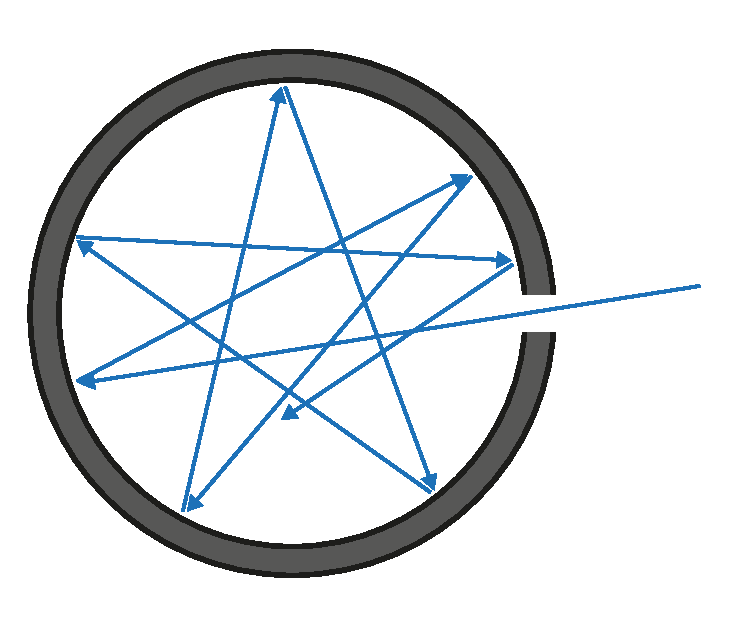
\includegraphics[width=0.5\linewidth]{figs/cuerpo-negro.pdf}
\caption{Modelo de Cuerpo Negro como una cavidad con un pequeño orificio a 
         través del cual ingresa la radiación electromagnética
         (\url{https://en.wikipedia.org/wiki/File:Black_body_realization.svg}).
         }
\label{fig:cuerpo-negro}
\end{figure}

La física clásica de finales del Siglo XIX proponía modelar el cuerpo negro 
como un conjunto de ondas electromagnéticas estacionarias dentro de la 
cavidad, a las cuales se les asignaba energías continuas, de acuerdo con la 
teoría electromagnética clásica conocida hasta el momento.
Sin embargo, los resultados teóricos no solo no coincidían con los 
obtenidos experimentalmente, sino que predecían lo que se conoce como la 
\emph{catástrofe ultravioleta}: las emisiones correspondientes a altas 
frecuencias debían aportar una enorme cantidad de energía, por lo que la 
energía total emitida por el cuerpo negro tendía a infinito.
Esto violaba los postulados de la conservación de la energía, poniendo en 
jaque la física clásica conocida hasta el momento.

Planck (1900) se vio forzado a introducir la hipótesis del quantum de 
energía, es decir, asignarle a cada onda electromagnética niveles de 
energías discretos, resolviendo el problema de la \emph{catástrofe 
ultravioleta} y concibiendo uno de los trabajos pioneros en lo que hoy 
conocemos como la mecánica cuántica.

En 1924, Bose modela la radiación dentro de la cavidad como un gas de 
fotones, y junto a los trabajos de Einstein (1924 y 1925) de reformulación y 
generalización de esta teoría, dan nacimiento a lo que hoy conocemos como la 
\emph{estadística de Bose-Einstein}.


\begin{enumerate}[label=(\alph*),
                  leftmargin=2\parindent,
                  rightmargin=2\parindent]

     \item{Consideremos un gas de fotones dentro de una caja de volumen $V$.
           La energía de cada fotón puede expresarse como:
           $$ \epsilon = \hbar \omega = c p , $$
           mientras que los autovalores de los momentos de cada uno de ellos 
           puede escribirse de la siguiente manera:
           $$
           p^2 = \frac{\pi^2 \hbar^2}{V^{2/3}}
           \left( n_x^2 + n_y^2 + n_z^2 \right), \quad
           n_x, n_y, n_z = 1, 2, 3, \dots .
           $$
           Dicha expresión de la energía de los fotones se debe a su propia 
           naturaleza, mientras que la discretización de los niveles de 
           energía viene dada por las condiciones de contorno en las paredes 
           de la cavidad.
           Obtener la siguiente expresión de  la energía por unidad de volumen 
           emitida por fotones con frecuencia entre $\omega$ y $\omega$ + 
           d$\omega$:
           $$
           u(\omega, T)d\omega = \frac{\hbar}{\pi^2 c^3}
           \frac{\omega^3}{e^{\beta \hbar \omega} - 1} d\omega
           $$
           Esta expresión se conoce como la fórmula de Planck de la 
           distribución de frecuencias de la densidad de energía del cuerpo 
           negro.
           }

     {\small
     \textbf{Ayuda:}
     El número de fotones $N$ dentro de la cavidad no es constante, ya que 
     son absorbidos y emitidos por las paredes internas.
     Sin embargo, si consideramos al sistema (cavidad + fotones) como aislado, 
     la entropía debe maximizarse:
     $$
     \left( \frac{\partial S}{\partial N} \right)_{E, V} =
     - \frac{\mu}{T} = 0 \quad \Rightarrow \quad \mu = 0.
     $$
     Por ende, podemos considerar que el gas de fotones posee potencial 
     químico nulo.
     }
     
     \item{Demostrar que en el límite de bajas frecuencias la fórmula de 
           Planck puede aproximarse por la distribución de Rayleigh-Jeans:
           $$ u(\omega, T) \propto \omega^2, $$
           o bien por la distribución de Wien:
           $$ u(\omega, T) \propto \omega^3 e^{\beta \hbar \omega}. $$
           Realizar una gráfica de las tres distribuciones (la de Planck, la 
           de Rayleigh-Jeans y la de Wien) en función de la frecuencia 
           $\omega$.
           Interpretar qué distribuciones predicen la catástrofe 
           ultravioleta y cuáles no.
           }
     
     \item{Calcular la ley de Stefan-Boltzmann a partir de la distribución 
           de Planck, es decir, demostrar que el valor medio de la energía 
           por unidad de volumen puede calcularse como:
           $$ U(T) = 4 \frac{\sigma}{c} T^4, $$
           determinar la \emph{constante de Stefan-Boltzmann} ($\sigma$) y su 
           valor.
           }
     
     \item{Calcular la presión de radiación, es decir, la presión que 
           ejerce el gas de fotones en las paredes internas de la cavidad, y 
           expresarla en función del valor medio de la energía por unidad de 
           volumen $U(T)$.
           }

\end{enumerate}

\end{document}

